\pdfoutput=1
\documentclass[11pt]{article}

\usepackage{acl}
\usepackage{times}
\usepackage{latexsym}
\usepackage[T1]{fontenc}
\usepackage[utf8]{inputenc}
\usepackage{microtype}
\usepackage{inconsolata}
\usepackage{graphicx}
\usepackage{booktabs}

\title{Report MNLP}
%\date{May $4^{th}$, 2025}

\author{Ercoli Fabio Massimo \\
\texttt{802397} \\\And
Della Porta Nicolò \\
\texttt{1920468} \\\And
Regina Giovanni \\
\texttt{1972467} \\}

\begin{document}

	\maketitle

	\section{Introduction}
	Cultural items are elements such as concepts or entities that carry cultural meaning and reflect the identity, practices, and values of specific communities. In natural language, these items can appear in diverse forms, ranging from food names and historical references to gestures and works of art. Their interpretation often depends on shared knowledge within a culture, making their automatic classification a complex task.
	In this report, it is described how we addressed the task of automatic cultural item classification. The goal is to label each item by identifying the category it belongs to among the three given categories: \textit{Cultural Agnostic (CA)}, \textit{Cultural Representative (CR)} and \textit{Cultural Exclusive (CE)}. As requested, to tackle this we implemented and evaluated two distinct approaches: a LM-based method using an encoder Transformer and a non-LM-based method relying on several data. The report presents a comparative analysis of the two approaches in terms of classification performance and it explains how they work by reflecting on the methodological choices employed.

	\section{Methodology}

	\subsection{Non-LM-based}
	The main idea is very simple: using a FF (feed forward) shallow neural network to classify the items, using the labels to implement a typical supervised learning. For each entity we provide different kinds of information, for instance the Wikidata description, the Wikipedia page text, but also the set of languages for which we have a Wikipedia page, the category of the item (provided by the Homework dataset), but also the set of claims (attributes) defined in the Wikidata entry.
	The Wikidata description text is used twice as input, as frequency vector and is transformed into GloVe embeddings. We provide both as input.
	
	For each of those elements we build a frequency vector that have different dimensions, so we're using different dictionaries having different sizes. The idea we had is to re-scale each of original vector size to values that can be parameterize, in particular those re-scaled values are hyper parameters of the solution. So for each input we produce an embedding, and we concatenate all of those to create the input of the classifier, that is as we said, a FF (feed forward) shallow neural network. Each input embedding is a function of an input.
	
	Decide how to scale the input looks crucial to us, since the original frequency vector sizes are very different and we want make each input contributing with the right weight in order to classify well the entities. 
	
	\subsection{LM-based}
	The solution is built around a pretrained encoder that generates embeddings, which serve as the input to the classification network. We tokenize both the Wikidata descriptions and the English Wikipedia pages, experimenting with several English-only encoders. After multiple trials, we selected RoBERTa-base as the encoder, limiting the number of training epochs to optimize validation set accuracy.

	\section{Experiments}
	We use only the training set to train the network, while the validation set helps us evaluate how well the model generalizes to unseen data. Since the dataset is relatively balanced across labels, we focused on maximizing validation accuracy.
	
	During training, for each epoch, we track the loss and accuracy on both the training and validation sets. In particular, we monitor validation accuracy over epochs to determine the optimal point at which to stop training.
	
	At inference time, we generate label predictions for the entire validation set and compute the overall accuracy. We also predict labels for the test set and compile the results into a CSV file, as required by the assignment.
	
	\section{Results}
	
	For the non-LM-based classifier at inference time we get an overall accuracy of 0.7533333333333333, matching 226 on 300 items. For the LM-based classifier at inference time we get an overall accuracy of 0.7966666666666666, matching 239 on 300 items. 

	\appendix
	
	\section{Training results Appendix}
	\label{sec:appendix}
	
	\begin{figure}
		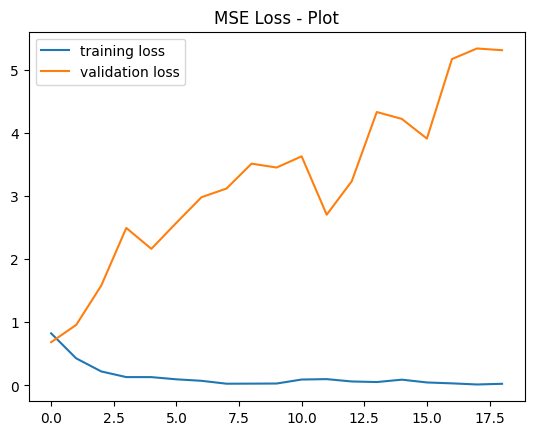
\includegraphics[width=\linewidth]{loss-no-transformer.png}
		\caption{non-LM-based classifier cross entropy loss.}
		\label{fig:1}
	\end{figure}
	
	\begin{figure}
		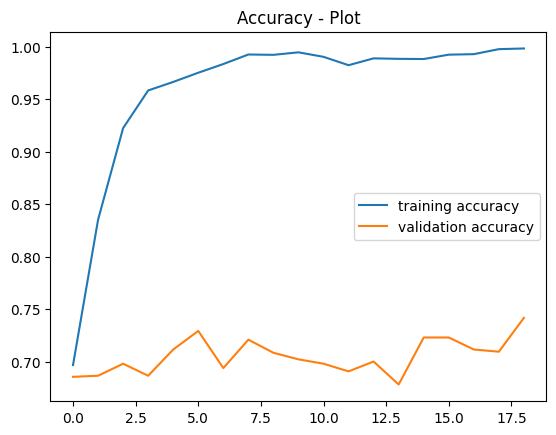
\includegraphics[width=\linewidth]{accuracy-no-transformer.png}
		\caption{non-LM-based classifier accuracy.}
		\label{fig:2}
	\end{figure}
	
	\begin{figure}
		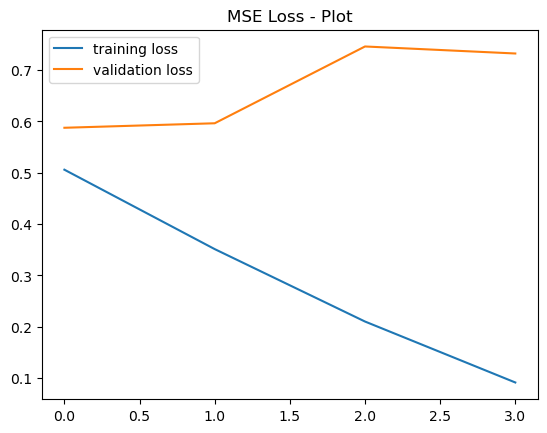
\includegraphics[width=\linewidth]{loss-yes-transformer.png}
		\caption{LM-based classifier cross entropy loss.}
		\label{fig:3}
	\end{figure}
	
	\begin{figure}
		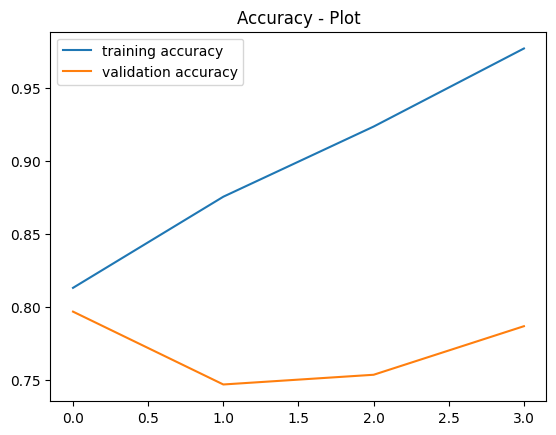
\includegraphics[width=\linewidth]{accuracy-yes-transformer.png}
		\caption{LM-based classifier accuracy.}
		\label{fig:4}
	\end{figure}
	
	Figure \ref{fig:1} ,  \ref{fig:2} ,  \ref{fig:3}  and  \ref{fig:4} present the cross entropy
	loss and accuracy for each epoch during the trainings.
	
	\begin{table}[]
		\begin{tabular}{@{}llll@{}}
			\toprule
			\multicolumn{1}{|l|}{train\_loss} & \multicolumn{1}{l|}{train\_accuracy} & \multicolumn{1}{l|}{valid\_loss} & \multicolumn{1}{l|}{valid\_accuracy} \\ \midrule
			4                                 & 4                                    & 4096                             &                                      \\
			32                                & 30                                   & 512                              &                                      \\
			32                                & 30                                   & 512                              &                                      \\
			32                                & 30                                   & 512                              &                                      \\
			32                                & 30                                   & 512                              &                                      \\
			32                                & 30                                   & 512                              &                                      \\
			32                                & 30                                   & 512                              &                                      \\ \cmidrule(r){1-3}
		\end{tabular}
	\end{table}
	
	\section{Tested encoder models}
	\label{sec:appendix}
	
	In the table we present the model we used for the LM-based classifier. 
	
	\begin{table}[]
		\begin{tabular}{@{}l|lll@{}}
			\toprule
			& \multicolumn{1}{l|}{batch\_size} & \multicolumn{1}{l|}{epochs} & \multicolumn{1}{l|}{length} \\ \midrule
			\multicolumn{1}{|l|}{google/bigbird-roberta-base} & 4                                & 4                           & 4096                             \\ \cmidrule(r){1-1}
			\multicolumn{1}{|l|}{distilbert-base-uncased}     & 32                               & 30                          & 512                              \\ \cmidrule(r){1-1}
			\multicolumn{1}{|l|}{roberta-base}                & 32                               & 30                          & 512                              \\ \cmidrule(r){1-1}
			\multicolumn{1}{|l|}{xlm-roberta-base}            & 32                               & 30                          & 512                              \\ \cmidrule(r){1-1}
			\multicolumn{1}{|l|}{xlm-roberta-large}           & 32                               & 30                          & 512                              \\ \cmidrule(r){1-1}
			\multicolumn{1}{|l|}{microsoft/mdeberta-v3-base}  & 32                               & 30                          & 512                              \\ \cmidrule(r){1-1}
			\multicolumn{1}{|l|}{microsoft/mdeberta-v3-large} & 32                               & 30                          & 512                              \\ \bottomrule
		\end{tabular}
	\end{table}
	
	\section{Algorithms  Appendix}
	\label{sec:appendix}
	
	Put the algorithms here.

\end{document}

